\section{计算空间距离}

\subsection{点到平面的距离}

\begin{theorem}
    点 $P$ 到平面 $A B C$ 的距离可以通过以下公式计算：
    \[
        d = \frac{|\overrightarrow{n} \cdot \overrightarrow{A P}|}{|\overrightarrow{n}|}
    \]
    其中，$\overrightarrow{n}$ 是平面的法向量，$\overrightarrow{A P}$ 是从平面上一点 $A$ 到点 $P$ 的向量。
\end{theorem}

\subsection{线面角与点面距的计算}

\begin{problem}
如图，在四棱柱 $A B C D-A_1 B_1 C_1 D_1$ 中，$A A_1 \perp$ 平面 $A B C D$ ，底面 $A B C D$ 是平行四边形，$A B=A D=B D=A A_1=2$ 。
\begin{enumerate}
    \item[(1)] 求直线 $B D_1$ 与平面 $A C D_1$ 所成角的正弦值；
    \item[(2)] 求点 $B_1$ 到平面 $A C D_1$ 的距离．
\end{enumerate}

\begin{figure} [H]
    \resizebox{0.2\textwidth}{!}{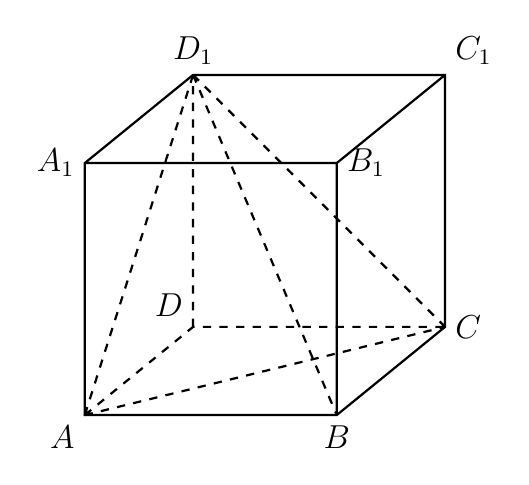
\begin{tikzpicture}[scale=.8,font=\large,thick]
\coordinate(A)at(0,0);\coordinate(B)at(4,0);\coordinate(C)at(5.72,1.4);\coordinate(D)at(1.72,1.4);\coordinate(A1)at(0,4);\coordinate(B1)at(4,4);\coordinate(C1)at(5.72,5.4);\coordinate(D1)at(1.72,5.4);
\draw(A)--(B)--(C)--(C1)--(D1)--(A1)--cycle (A1)--(B1)--(C1) (B)--(B1);
\draw[dashed](A)--(D)--(C) (D)--(D1) (D1)--(A) (D1)--(B) (D1)--(C) (A)--(C);
\foreach\p/\pos in{A/below left,B/below,C/right,D/above left}{\node[\pos]at(\p){$\p$};}\node[left]at(A1){$A_1$};\node[right]at(B1){$B_1$};\node[above right]at(C1){$C_1$};\node[above]at(D1){$D_1$};
\end{tikzpicture}
}
\end{figure}

\end{problem}

\subsection{平行平面的距离}

\begin{theorem}
    以上，直接转化为点到平面的距离就能算了。
\end{theorem}

\begin{example}
    在棱长为 2 的正方体 $A B C D-A_1 B_1 C_1 D_1$ 中，求
    \begin{enumerate}
        \item 直线 $B C$ 与平面 $A B C_1 D_1$ 所成的角；
        \item 求平面 $A_1 B D$ 与平面 $B_1 D_1 C$ 的距离；
        \item 求三棱雉 $B_1-A_1 B D$ 外接球的表面积；
    \end{enumerate}
\end{example}

\begin{figure} [H]
    \resizebox{0.2\textwidth}{!}{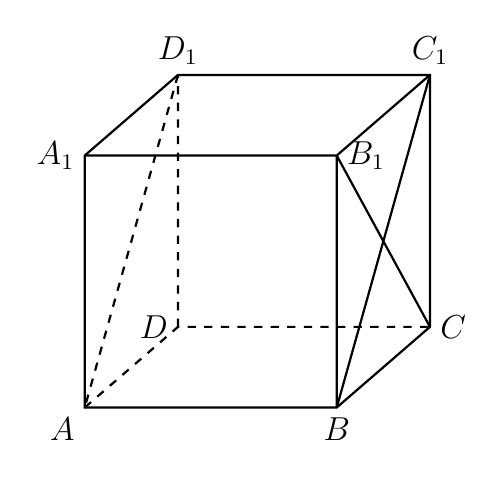
\begin{tikzpicture}[scale=.8,font=\large,thick]
\coordinate(A)at(0,0);\coordinate(B)at(4,0);\coordinate(C)at(5.48,1.28);\coordinate(D)at(1.48,1.28);\coordinate(A1)at(0,4);\coordinate(B1)at(4,4);\coordinate(C1)at(5.48,5.28);\coordinate(D1)at(1.48,5.28);
\draw(A)--(B)--(C)--(C1)--(D1)--(A1)--cycle (A1)--(B1)--(C1) (B)--(B1);\draw(C1)--(B) (B1)--(C);
\draw[dashed](A)--(D)--(C) (D)--(D1) (D1)--(A);
\foreach\p/\pos in{A/below left,B/below,C/right,D/left}{\node[\pos]at(\p){$\p$};}\node[left]at(A1){$A_1$};\node[right]at(B1){$B_1$};\node[above]at(C1){$C_1$};\node[above]at(D1){$D_1$};
\end{tikzpicture}
}
\end{figure}

\subsection{点到直线的距离}

\begin{theorem}

\end{theorem}

\subsection{异面直线的距离}

\begin{definition}
    两条异面直线之间的距离是指其中一条直线上任意一点到另一条直线距离的最小值。
\end{definition}

\begin{theorem}
    $AB$为异面直线 $a$、$b$ 的公垂线段，$\overrightarrow{n}$ 为直线$AB$的方向向量，$E$、$F$分别为直线 $a$、$b$ 上的任意一点，则
    \[
        |AB| = \frac{|\overrightarrow{EF} \cdot \overrightarrow{n}|}{|\overrightarrow{n}|}
    \]
\end{theorem}

\begin{figure}[h!]
    \centering
    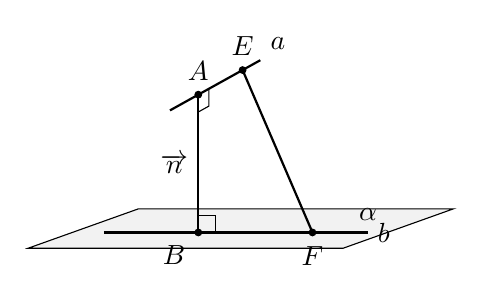
\begin{tikzpicture}[
            scale=1,
            x={(1cm,0cm)},
            y={(0.45cm,0.25cm)},
            z={(0cm,1cm)},
            point/.style={circle, fill=black, inner sep=1pt}
        ]
        \coordinate (P1) at (-1.8,-0.8,0);
        \coordinate (P2) at (2.2,-0.8,0);
        \coordinate (P3) at (2.7,1.2,0);
        \coordinate (P4) at (-1.3,1.2,0);
        \coordinate (B) at (0,0,0);
        \coordinate (F) at (1.45,0,0);
        \coordinate (A) at (0,0,1.75);
        \coordinate (E) at (0,1.25,1.75);

        \draw[fill=gray!10] (P1) -- (P2) -- (P3) -- (P4) -- cycle;
        \node at (1.75,0.9,0) {$\alpha$};
        \draw[thick] (0,-0.8,1.75) -- (0,1.75,1.75) node[above right] {$a$};
        \draw[thick] (-1.2,0,0) -- (2.15,0,0) node[right] {$b$};
        \draw[thick] (A) -- (B) node[midway, left] {$\overrightarrow{n}$};
        \draw[thick] (E) -- (F);

        \node[point, label=above:$A$] at (A) {};
        \node[point, label=below left:$B$] at (B) {};
        \node[point, label=above:$E$] at (E) {};
        \node[point, label=below:$F$] at (F) {};
        \draw (B) ++(0.22,0,0) -- ++(0,0,0.22) -- ++(-0.22,0,0);
        \draw (A) ++(0,0.3,0) -- ++(0,0,-0.22) -- ++(0,-0.3,0);

    \end{tikzpicture}
    \caption{异面直线公垂线段示意图}
    \label{fig:skew_lines}
\end{figure}

% --- 证明过程 ---
\begin{proof}
    显然 $\overrightarrow{AB} = \overrightarrow{AE} + \overrightarrow{EF} + \overrightarrow{FB}$，
    因为 $\overrightarrow{n}$ 是公垂线 $AB$ 的方向向量，所以 $\overrightarrow{n} \perp a$ 且 $\overrightarrow{n} \perp b$。
    又因为 $\overrightarrow{AE}$ 在直线 $a$ 上，$\overrightarrow{FB}$ 在直线 $b$ 上，所以 $\overrightarrow{AE} \perp \overrightarrow{n}$，$\overrightarrow{FB} \perp \overrightarrow{n}$。
    因此，它们的点积为零：
    \[ \overrightarrow{AE} \cdot \overrightarrow{n} = 0, \quad \overrightarrow{FB} \cdot \overrightarrow{n} = 0 \]
    所以，我们将 $\overrightarrow{AB}$ 与 $\overrightarrow{n}$ 作点积：
    \[
        \overrightarrow{AB} \cdot \overrightarrow{n} = (\overrightarrow{AE} + \overrightarrow{EF} + \overrightarrow{FB}) \cdot \overrightarrow{n}
    \]
    \[
        \overrightarrow{AB} \cdot \overrightarrow{n} = \overrightarrow{EF} \cdot \overrightarrow{n}
    \]
    两边取绝对值：
    \[
        |\overrightarrow{AB} \cdot \overrightarrow{n}| = |\overrightarrow{EF} \cdot \overrightarrow{n}|
    \]
    \[
        |AB| = \frac{|\overrightarrow{EF} \cdot \overrightarrow{n}|}{|\overrightarrow{n}|}
    \]
\end{proof}
